% preambula dokumenta
\documentclass[a4paper, 10pt]{article}
\usepackage[slovene]{babel}
\usepackage[utf8]{inputenc}
\usepackage[T1]{fontenc}
\usepackage{lmodern}
\usepackage[pdftex]{graphics}
\usepackage{amsmath}
\usepackage{graphicx}
\usepackage{eurosym}
\usepackage{float}
\graphicspath{ {./images/} }

\renewcommand*\contentsname{Kazalo}
\pagenumbering{arabic}

% telo dokumenta
\begin{document}

\begin{titlepage}
\begin{center}

\Huge 
\textbf{Predpostavka o Randićevem indeksu in radiusu}

\vspace{1cm}
\Large
\textbf{Poročilo pri predmetu Finančni praktikum}

\vspace{1cm}

\vspace{2,5cm}
\large
Avtorja:\\
\textbf{Jaka Munda, Anja Žavbi Kunaver}\\

\vfill

\Large Ljubljana, januar 2019

\end{center}
\end{titlepage}

\tableofcontents

\pagebreak

\section{Opis problema}
Računalniški program Graffiti je postavil lemo, da za enostaven povezan graf $G=(V, E)$ velja, $$ Ra(G) \geq rad(G) -1.$$
Domnevo je potrebno testirati na različne načine na manjših in večjih grafih.
Z uporabo metahevristične populacije je domnevo potrebno preizkusiti na večjih grafih in upati na njeno ovrgbo.

\subsection*{Opombe:}
\begin{enumerate}
\item Graf je enostaven, če ne vsebuje zank in je brez vzporednih povezav.
\item Graf je povezan, če lahko iz vsake točke pridemo do vsake druge točke v grafu.
\item Ekscentričnost vozlišča $v$ je razdalja do njegovega najbolj oddaljenega vozlišča; tj. $\max \{d(v,u) : u \in V(G) \}$.
\item Radius grafa $rad(G)$ pomeni minimum ekscentričnosti vozlišč grafa.
\item $Ra(G)$ je Randićev indeks grafa G. Definiran je kot
$$Ra(G) = \sum_{uv \in E(G)} \frac{1}{\sqrt{d(u) d(v)}}.$$
\item $d(x)$ predstavlja stopnjo vozlišča $x$ oz. število povezav, ki imajo vozlišče $x$ za svoje krajišče.
\end{enumerate}

\section{Potek dela}

Programiranje sva opravila v programu Sage, ki ima že vgrajene funkcije za delo z grafi.
Najprej sva napisala program, ki je lemo testiral na manjših enostavnih povezanih grafih. S tem programom sva uspela lemo potrditi za grafe s številom vozlišč $n \leq 9$. Za grafe z večjim številom vozlišč pa program ni deloval, zato sva se dela lotila z metodo populacijske metahevristike, in sicer z genetskim algoritmom.

\pagebreak
\section{Primer}
Za lažje razumevanje prilagava primer enostavnega povezanega grafa s 5 vozlišči.

\begin{align*}
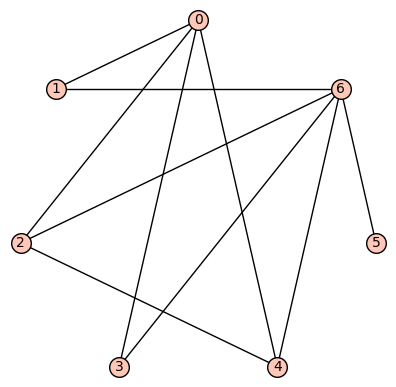
\includegraphics{primer}
\end{align*}

$$radius = 2$$
$$Ra(G) = \frac{1}{\sqrt{4}} + \frac{1}{\sqrt{6}} + \frac{1}{\sqrt{6}} + \frac{1}{\sqrt{6}} + \frac{1}{\sqrt{6}} + \frac{1}{\sqrt{9}} = \frac{5+4\sqrt{6}}{6} \doteq 2.47$$

\vspace{0.5cm}
Vidimo, da na tem grafu lema drži, saj je $2.47 > 2 - 1$.

\section{Algoritem za manjše grafe}
Najprej sva definirala funkcijo, ki za graf vrne Randićev indeks po definirani formuli. Funkcija za izračun radiusa grafa je že vgrajena.
Nato sva definirala funkcijo, ki za vse grafe velikosti $n$ in manj preveri, ali domneva drži. V kolikor lema za kakšen graf ne bi držala, bi funkcija vrnila $False$, vendar pa se to v nobenem primeru ni zgodilo. Ta funkcija deluje za grafe do števila vozlišč $n \leq 9$.

\pagebreak
\section{Algoritem za večje grafe}
\

Z genetskim algoritmom sva poskušala ovreči domnevo.
Ponovno sva najprej definirala Randićev indeks, enako kot pri majhnih grafih.

Nato sva definirala funkcijo fitness, ki vrne vrednost neenakosti, torej $Ra(G)-rad(G)+1$. Če bi vrnila negativno vrednost, bi bila lema ovržena.

Naslednja funkcija $tournament\_selection$  med t naključno izbranimi grafi izbere tistega, ki ima najmanjšo vrednost funkcije fitness. Najprej naključno izbere enega izmed grafov in ga spravi v `najbolsi', nato pa pregleduje ostale grafe in če najde boljšega, ga zamenja.

Definirala sva funkcijo za Poissonovo porazdelitev, ki pride v poštev kasneje. Z njo bomo izbirali število povezav, ki jih bomo v funkciji $mutiraj$ odstranili oziroma dodali. V funkciji $crossover$ nam pove, koliko povezav bomo dodali potomcu.

Funkcija $mutiraj$ prejme graf in ga mutira. To naredi tako, da najprej naključno izbere neko verjetnost. Če je ta verjetnost $\leq\frac{1}{3}$, doda povezavo, če je  $> \frac{1}{3}$ in $\leq \frac{2}{3}$, odstrani povezavo in če je $> \frac{2}{3}$, doda in odstrani povezavo.

$crossover$ prejme dva grafa in ju križa med seboj ter vrne njunega potomca.

$min\_fitness$ prejme seznam grafov, med katerimi poišče tistega, ki ima najmanjšo vrednost funkcije $fitness$. To pa zato, ker manjša kot je ta vrednost, večja je verjetnost, da bo lema ovržena. Želiva namreč priti pod vrednost 0, večje vrednosti pa lemo le potrdijo za en določen graf.

S funkcijo $nova\_populacija$ iz obstoječe populacije narediva novo populacijo s pomočjo križanja in mutacij.

Še zadnja funkcija $genetic\_algorithm$ v vsaki ponovitvi s križanjem in mutiranjem naredi novo populacijo. Če v tej populaciji najde graf, za katerega je vrednost $fitness$ manjša od nič, vrne `Lema ne drži'. Če se to ne zgodi pri nobenem grafu, vrne `Ne najdem protiprimera'. Lemo sva nato testirala z vnašanjem različnih vrednosti v zadnjo funkcijo in ob tem beležila čase delovanja.

\section{Ugotovitve}
Ugotovila sva, da imajo polni grafi z več kot enim vozliščem radius vedno enak 1. Iz tega dokaj očitno sledi, da neenakost velja (celo stroga neenakost).
Tudi z genetskim algoritmom pa nama ni uspelo najti protiprimera. Morda bi uspelo s kakšnimi drugimi vhodnimi podatki.
Na podlagi tega leme ne moreva ovreči ali potrditi v celoti.

\pagebreak

\section{Literatura}
\vspace{0.5cm}

\renewcommand{\labelenumi}{[\arabic{enumi}]}
\begin{enumerate}
\item \noindent M. Cygan, M. Pilipczuk, R. Škrekovski, \textsl{On the Inequality between Radius and Randic Index for Graphs}, 2011. 
\vspace{0.5cm}
\item \noindent  S. Luke, \textsl{Essentials of Metaheuristics}, Department of Computer Science, George Mason University, Online Version 2.2, 2015.
\end{enumerate}

\end{document}
